\subsection{Challenges}
  \subsubsection{Filtered emails}
    One big design challenge we faced was how to reduce the number of irrelevant emails a student was receiving. Two solutions that were not optimal were discussed:
    \begin{itemize}
      \item \textbf{Opt in emails:} Students could opt in for receiving certain email categories based on tags. We soon realised that this would require a lot of maintenance by students to continuously update their whitelist with tags as they were being created.
      Not only would it be a lot of work for a student, but students might miss out on exciting emails which do not fall into specific categories, or a category a student had remembered to whitelist. For example the Raspberry Pi is unlikely to fall into a tag group but it's own. If a student forgets to add this to their list they'll miss out entirely on the emails when the likelihood is that they may have been interested.
      \item \textbf{Opt out emails:} Students can blacklist tags that they never want to hear from. If an email contains a tag that a student has blacklisted then the student will never get sent this email. Whilst this is a lot closer to our ideal solution we still have the case of a student being interested in C++ say and choosing to blacklist Java. If an email contains two sections about these two languages and is labeled with both tags the student will never receive the email since Java was in their blacklist.
    \end{itemize}

    We have therefore devised a hybrid solution:
    \begin{itemize}
      \item A student will \textbf{receive} an email if none of the email tags fall in a students blacklist.
      \item A student will \textbf{receive} an email if one or more email tags fall in their blacklist but a tag in the emails list exists in their skill set.
      \item A student will \textbf{not receive} emails from a company they have blocked unless they have signed up to an event in which case they will \textbf{receive} the event related emails only.
      \item A student will \textbf{not receive} an email if any of the tags exist in the emails tags and none exist in the students skill set.
    \end{itemize}

    Furthermore in the student account settings we allow them to choose between receiving this smart email system, all emails, or only personal and event emails.

  \subsubsection{Intuitive Features}
    Since it is not feasible to write a user manual for a website we faced many challenges ensuring that each user finds our site easy to navigate through and is made aware very quickly about the features that are available to them. Since we developed the site it is obvious to us how to use it but to ensure that users know too we have made use of the following:

    \paragraph{Tooltips:} These appear whenever you run your cursor over an area of text that can be edited in place, or over features that might not be completely obvious (such as company contact card drag and drop). Examples are the student's name, year, degree, and bio. They all start with `click to' and we believe they are well placed and helpful rather than irritating.      
    \begin{figure}[H]\centering
    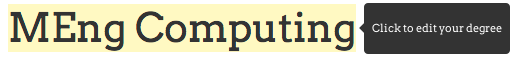
\includegraphics[scale=0.5]{images/design/edit_degree_tooltip}
    \caption{Useful degree tooltip}
    \end{figure}
    Tooltips also appear throughout for both company and department administrators.
    Once a user is comfortable with using the site, they have the option to turn tooltips off in their settings.

    \paragraph{Yellow Highlighting:} This also ties in nicely with the tooltips and highlights the boundary for what can and cannot be edited.

    \paragraph{Incomplete Sections:} In order to highlight a section, document or field that is incomplete we have opted to colour these in red rather than providing a message. We feel that by keeping this theme consistent throughout all users profiles it is quite intuitive in itself.
    What's more is that when a student initially signs up they are informed that their profile is invisible and they need to fill in certain fields before it will be shown to companies. As they fill in these fields (which are initially red) the colour disappears and we hope that students will intuitively learn from the beginning that the red colouring means an item is missing. The same can be said for companies.

    \paragraph{Typeahead} Unfortunately there are too many degree types throughout departments for us to validate them all. For example just within the Department of Computing we have BEng, MEng, PhD, MSc and within these we have specialist titles such as Artificial Intelligence, Software Engineering, Computation in Biology and Medicine etc.\cite{doc-ug-degrees}. In order to achieve our objective of being available to produce a product for multiple departments it is just not possible to validate these. Therefore in order to try to ensure students doing the same degree have the same title (i.e. `MEng Computing' rather than `MEng computing' or `meng computing' etc.) we have used Twitter Bootstrap's\cite{bootstrap} typeahead feature which provides options for students to choose from on typing. They will hopefully feel encouraged to click on these option which are populated from the list of degrees that students throughout the department are currently using on their profiles and so is very dynamic.

    \begin{figure}[H]\centering
    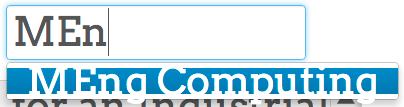
\includegraphics[scale=0.5]{images/design/edit_suggestions}
    \caption{Drop down degree suggester}
    \end{figure}

    Likewise we make use of typeaheads throughout our site when allowing tag input. The aim of this is to make users aware of the tags available to them on input. This is again dynamically populated from the list of student's tags, and if a tag is not in the list, students have the option to add a new one by simply typing it in the tag input field. 

    We decided that only students should be allowed to add new tags - companies can only tag their emails with ones that exist in the system. This aids in the smart email filtering and ensures companies cannot use a tag that no students have expressed a skill or interest in.
    All tags are automatically downcased both on the server and the client to avoid duplication.

    \paragraph{Navigation:} This has largely been made possible through the use of a navigation bar at the top of our website. We feel that this is intuitive to all of our users who will be familiar with navigation bars from other sites such as Facebook\cite{facebook}, LinkedIn\cite{linkedin} and even Google\cite{google}. These websites really encourage user interaction by clicking on items located anywhere on the page and adopt the technique of changing the cursor to a pointer (hand) rather than the default which is normally displayed when you can interact with an object. As such we've adopted this technique throughout our site when items on the page can be clicked to redirect. For example students can click on the top three events and placements that are displayed on their dashboard. In order to make it very obvious we subtly change the colour scheme of the background to display that they've highlighted it.
    % TODO INSERT PICTURE HERE

    We have also made use of icons in order to make navigation more intuitive, again users of every day websites have become accustomed to certain items meaning certain things, for example a cog is often associated with settings and so we had no qualms about using them freely in the design of our site.
    The downwards facing caret is used to alert users that clicking on their name on the navigation bar provides them with extra options.
    
    \begin{figure}[H]\centering
    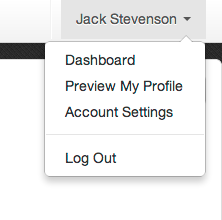
\includegraphics[scale=0.5]{images/design/navigation_caret}
    \caption{Drop down menu, intention aided by dropdown caret}
    \end{figure}

    Similarly the star and ban icons on a company as featured earlier, combined with the tooltips make it clear to a user what they mean.

    \begin{figure}[H]\centering
    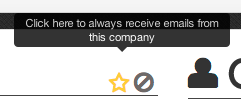
\includegraphics[scale=0.5]{images/design/company_star}
    \caption{Tooltip for favouriting a company}
    \end{figure}

  % IS #256 done?? THEN WE COULD WRITE HERE.
  \subsubsection{Multi Departmental}
    In order to make our system available to other departments we faced a couple of design decisions throughout the duration of our project.
    \begin{itemize}
      \item  The first decision was to allow students and company administrators to be part of multiple departments. Although this requires a little more logic for us it more than pays of for our users. For example when company administrators want to be part of multiple departments, we can now no longer expect them to specify all on sign up and must provide facilities for them to do this at a later date. If they were part of only one department we could have enforced it on sign up. However it would be very off putting if we forced them to create a new account for each department they were a member of.

      We also allow companies to create events for one or more of their registered departments through the use of a check box on the creation forms. We hope that this will ensure that there is no frustration of having to create the same form multiple times if it is relevant to a variety of departments. It also offers more flexibility than publishing the events and placements for every department a company is a member of.

      We then had to ensure that company administrators could request, on behalf of their company, access to other departments once they'd signed up. There are two reasons for this; firstly they may not know at sign up that they'd be interested in a particular departments students and secondly a department might start using the system once they'd already signed up. In order to do this we allow students to request new departments that are available. They will not have access to that department until a department administrator has logged in and given them approval and if they are rejected it is up to the administrator to email them to explain why. 
      
      \item Another challenge that arose was trying to decide what features other departments might like, and if anything we were creating was accidentally too specific to the Department of Computing. Although we were not willing to cater for specific departmental requests we wondered if there may have been something really generic we were missing.

      In order to overcome this challenge our supervisor, Will Knottenbelt, made us aware of a college wide meeting that was due take place on 21st November 2012. Unfortunately we could not make it in person because all members of the group had a lecture that morning so we decided to send him along with some screen shots and mock ups of our website. To our delight the feedback from the meeting was very positive with many departments saying that they very much liked what they'd seen. 
      
      We therefore set up a meeting with Clare Drysdale from the EEE department, who had been present at the meeting, to give her a live demo and gather her feedback. We chose the EEE department because they are in their second year of offering optional industrial placements as part of their MEng third year course and so Clare was likely to have a few ideas of things she wanted from her experience the previous year. In our meeting we found out that Clare was actually looking for a system to manage industrial placements, which is slightly different to CPP: Connect's objectives. As this would also be a very useful feature for Serena Coultress this would be an excellent extension to our project, although we had do decide as a group we could not implement this for the deadline since we did not have enough time to do the entire system justice.
      
      Even though the meeting with Clare did not have the outcome we'd hoped for she did stress that she very much liked the event and placement advertisements and would consider a trial run for the academic year of 2013-2014.

      \item Finally in order to not make our website too specific to any single department we had to leave the events and placement forms as general as possible. Therefore we opted to use a notification system in order to achieve our this objective. As seen previously, department administrators can set a note that will appear on the top of forms with any extra content they may need.
    \end{itemize}
   

    